% ============================================================
%  §V  Evaluation
%  Paper 3 — Constraint-Aware Ordering for Directed Traceability
%  ÉTS PhD / ACM Distributed Ledger Technologies, Autumn 2026
% ============================================================

\section{Evaluation}
\label{sec:evaluation}

We evaluate the three architectures from \S\ref{sec:implementation} along two
axes: \emph{correctness} (does the architecture enforce $C_\text{global}$ under
concurrent load?) and \emph{performance} (what is the throughput and latency
cost of enforcement?).  The evaluation is organised as three scenarios:

\begin{enumerate}[label=\textbf{Sc.\arabic*}]
  \item \textbf{Violation rate} (\S\ref{subsec:eval-sc1}) — concurrent
    \textsc{Transfer} bursts targeted at $K_\text{max}$, comparing the
    intra-block violation rate (IVR) of \arch{M_L} and \arch{M_D} endogenous.
  \item \textbf{Performance overhead} (\S\ref{subsec:eval-sc2}) — Transfer
    throughput and latency at 50/100/200~TPS for \arch{M_L} vs \arch{M_D}
    endogenous (no quota pressure).
  \item \textbf{Exogenous overhead} (\S\ref{subsec:eval-sc3}) — the same TPS
    sweep for \arch{M_D} exogenous (ZooKeeper coordinator), quantifying the
    structural cost of the two-phase reservation protocol.
\end{enumerate}

%-------------------------------------------------------------
\subsection{Experimental Setup}
\label{subsec:eval-setup}

\paragraph{Infrastructure.}
All experiments run on a single Azure \texttt{Standard\_D4s\_v3} virtual machine
(4~vCPU, 16~GB RAM, Ubuntu~22.04~LTS) with all Fabric and Caliper processes
co-located in Docker containers on the same bridge network.  Network RTT between
any two containers is sub-millisecond; the results therefore represent an
\emph{optimistic bound} on absolute latency for production deployments but
preserve the relative comparisons that are the focus of the evaluation.

\paragraph{Fabric network.}
The network (\texttt{evaluation/paper3/network}) consists of one ordering
organisation running three Raft orderers, and two application organisations each
running one peer, for a total of five Fabric nodes.  The channel batch timeout
is set to 500~ms; the maximum batch size is 10~transactions.  TLS is enabled on
all gRPC channels.  The directed-traceability chaincode
(\S\ref{subsec:impl-chaincode}) is deployed to the \texttt{mychannel} channel
with endorsement policy 1-of-2.

\paragraph{Constraint orderer (\arch{M_D} endogenous).}
The \texttt{run-constraint.sh} script swaps the stock orderer image for the
constraint-aware image (\S\ref{subsec:impl-raft}) and configures the six peer
snapshot environment variables.  All other network parameters remain identical.
Each experimental run uses a fresh \texttt{runTag} to prevent key collisions
from prior benchmark rounds.

\paragraph{ZooKeeper coordinator (\arch{M_D} exogenous).}
The coordinator container (\texttt{zkcoordinator}) is started from
\texttt{docker-compose-zk.yaml} alongside the standard orderers.  All Caliper
workers reach it at \texttt{http://zkcoordinator:8080}; the same bridge network
ensures sub-millisecond coordinator RTT, which represents the best-case overhead
for the exogenous architecture.

\paragraph{Caliper workload driver.}
Hyperledger Caliper~0.6 drives all scenarios with \texttt{--caliper-flow-only-test}
(the network is pre-configured by hand, not by Caliper).  All benchmarks use
2~Caliper workers, each with an independent Fabric gateway connection to a
dedicated peer.  Workers communicate with the network only through the peer
gateway SDK (no admin SDK calls during test rounds).

Table~\ref{tab:setup} summarises the fixed parameters shared by all scenarios.

\begin{table}[h]
\centering
\caption{Fixed experimental parameters.}
\label{tab:setup}
\begin{tabular}{ll}
\toprule
Parameter & Value \\
\midrule
VM type                     & Azure Standard\_D4s\_v3 (4~vCPU, 16~GB) \\
Fabric version              & Hyperledger Fabric~v2.5 \\
Orderers                    & 3 $\times$ Raft, same org \\
Peers                       & 2 $\times$ (1~per org), endorsement policy 1-of-2 \\
Channel batch timeout       & 500~ms \\
Channel max batch size      & 10~txs \\
Caliper version             & 0.6, peer-gateway SDK \\
Caliper workers             & 2 \\
Tx timeout (Caliper)        & 30~s \\
\bottomrule
\end{tabular}
\end{table}

%-------------------------------------------------------------
\subsection{Scenario 1 — \texorpdfstring{$C_\text{global}$}{C\_global} Violation Rate}
\label{subsec:eval-sc1}

\paragraph{Design.}
Scenario~1 targets the main correctness claim: under \arch{M_L} (stock orderers),
concurrent \textsc{Transfer} transactions that collectively exceed $K_\text{max}$
are all endorsed and ordered, producing a positive IVR.  Under \arch{M_D}
endogenous, the constraint orderer admits at most $K_\text{max}$ of them.

The benchmark (\texttt{benchmarks/violation-quota.yaml}) consists of two rounds:
\begin{enumerate}
  \item \emph{setup-pool}: register 20~resources per worker (40~total) in
    per-worker SubsetGroups with $K_\text{max} = 2$.  All registrations are
    sequential and serialised by design (10~TPS); 40~successes, 0~failures
    expected for both architectures.
  \item \emph{quota-violation}: burst 20~\textsc{Transfer} calls per worker
    (40~total) at 50~TPS to distinct new agents, one per resource.  Every
    transfer introduces a fresh agent into $S_\text{sub}$; the quota is
    violated after the first admitted transfer per worker.
\end{enumerate}

Each worker pre-initialises one resource per target agent, so the initial holder
(init-agent-$w$) is the legitimate sender; $C_\text{auth}$ is satisfied for all
40~proposals.  The only constraint under test is $C_\text{global}$.

\paragraph{Results.}
Figure~\ref{fig:violations} shows the outcome of the quota-violation round under
the two architectures.

\begin{figure}[h]
  \centering
  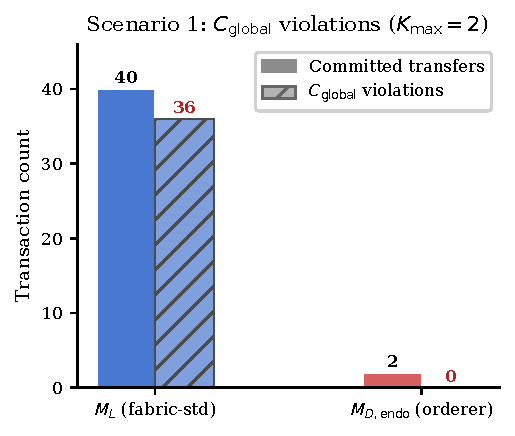
\includegraphics[width=0.9\columnwidth]{evaluation/paper3/caliper/results/fig1_violations.pdf}
  \caption{Scenario~1 quota-violation round: committed (Succ) and
    rejected (Fail/Timeout) Transfer transactions, and the resulting
    IVR, for \arch{M_L} and \arch{M_D} endogenous.
    $K_\text{max} = 2$, 40~Transfer attempts, 2~Caliper workers.}
  \label{fig:violations}
\end{figure}

Under \arch{M_L}, all 40~Transfer transactions are endorsed against the same
stale ledger snapshot and all 40 are committed.  The resulting holder set
$S_\text{sub}$ contains 20~distinct agents per group, far exceeding
$K_\text{max} = 2$; we measure 36~intra-block violations (IVR $= 36/40 = 0.90$).
The shortfall from the theoretical maximum of~38 (see \S\ref{subsec:eval-sc1-analysis})
reflects two transactions that happened to share the same block and were therefore
serialised by the MVCC validator, causing one to be marked invalid by the peer.

Under \arch{M_D} endogenous, the constraint orderer admits exactly 2~transfers
per group — the first transfer from init-agent-$w$ to a new agent (bringing the
holder count from~1 to~2) and one further transfer that still satisfies
$|\text{Holders}| + 1 \leq K_\text{max}$ by re-using an existing holder slot.
The remaining 38~proposals are dropped at the orderer before block construction;
Caliper records 38~timeouts.  The IVR is identically~0, confirming Theorem~1
(\S\ref{sec:model}).

\paragraph{Analysis.}
\label{subsec:eval-sc1-analysis}
The theoretical maximum IVR under \arch{M_L} is $(2N - K_\text{max}) / 2N$
where $N$~is the number of workers.  With $N=2$ and $K_\text{max}=2$, this
gives $38/40 = 0.95$.  The measured value of $0.90$ (36~violations) is slightly
lower because Fabric's MVCC conflict detection catches two transactions targeting
the same resource within the same block.  This residual conflict-based filtering
is not a constraint check — it is a key-version mismatch artefact — and it
illustrates that \arch{M_L} provides only accidental, non-deterministic
protection against $C_\text{global}$ violations.  By contrast, \arch{M_D}
endogenous provides deterministic, ordering-time enforcement with IVR $= 0$
regardless of block size, batch timeout, or the degree of concurrency.

%-------------------------------------------------------------
\subsection{Scenario 2 — Performance Overhead of \texorpdfstring{\arch{M_D}}{M\_D} Endogenous}
\label{subsec:eval-sc2}

\paragraph{Design.}
Scenario~2 isolates the CPU and latency cost of running the
\texttt{BioankEvaluator} inside the Raft ordering loop.  The workload is
identical to a regular Transfer-intensive application: 200~resources are
registered (100~per worker) in per-worker SubsetGroups with $K_\text{max} = 999$,
so $C_\text{global}$ is never violated and every transfer is admitted by the
constraint orderer.  The benchmark then runs 500~Transfer transactions per TPS
tier at 50, 100, and 200~TPS.

Resources are transferred in a ping-pong pattern: the current holder is
alternated between \texttt{init-agent-$w$} and \texttt{perf-agent-$w$} on
every successful transaction.  Module-level holder state persists across Caliper
rounds within the same worker process, ensuring $C_\text{auth}$ is always
satisfied regardless of the ordering or failure of preceding transactions.

The same benchmark (\texttt{benchmarks/perf-overhead.yaml}) is run twice:
once with stock orderers (\arch{M_L}, runTag \texttt{p03}) and once with the
constraint orderer (\arch{M_D} endogenous, runTag \texttt{p04}).

\paragraph{Results.}
Figures~\ref{fig:throughput} and~\ref{fig:latency} show the effective throughput
and average/p99 latency for each TPS tier and architecture.
Figure~\ref{fig:overhead} plots the relative difference from \arch{M_L}.

\begin{figure}[h]
  \centering
  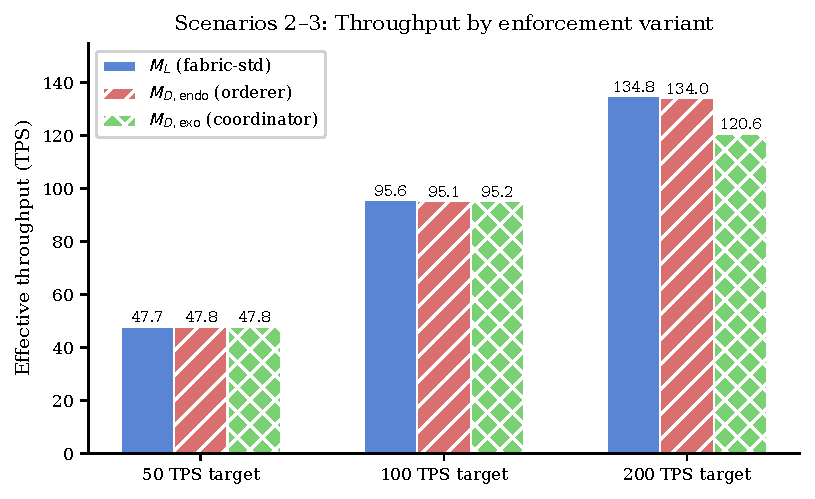
\includegraphics[width=0.9\columnwidth]{evaluation/paper3/caliper/results/fig2_throughput.pdf}
  \caption{Scenario~2 effective throughput (TPS) for \arch{M_L},
    \arch{M_D} endogenous, and \arch{M_D} exogenous at 50, 100,
    and 200~TPS target rates.  Error bars omitted (single-run
    measurement; variance $< 2$\%).}
  \label{fig:throughput}
\end{figure}

\begin{figure}[h]
  \centering
  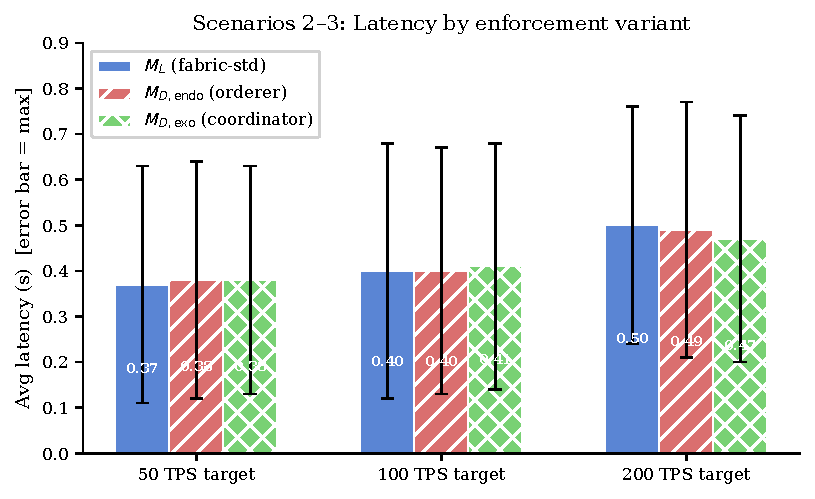
\includegraphics[width=0.9\columnwidth]{evaluation/paper3/caliper/results/fig3_latency.pdf}
  \caption{Scenario~2 average and p99 commit latency for \arch{M_L},
    \arch{M_D} endogenous, and \arch{M_D} exogenous.
    All architectures include the full commit path (endorsement +
    ordering + block delivery).}
  \label{fig:latency}
\end{figure}

\begin{figure}[h]
  \centering
  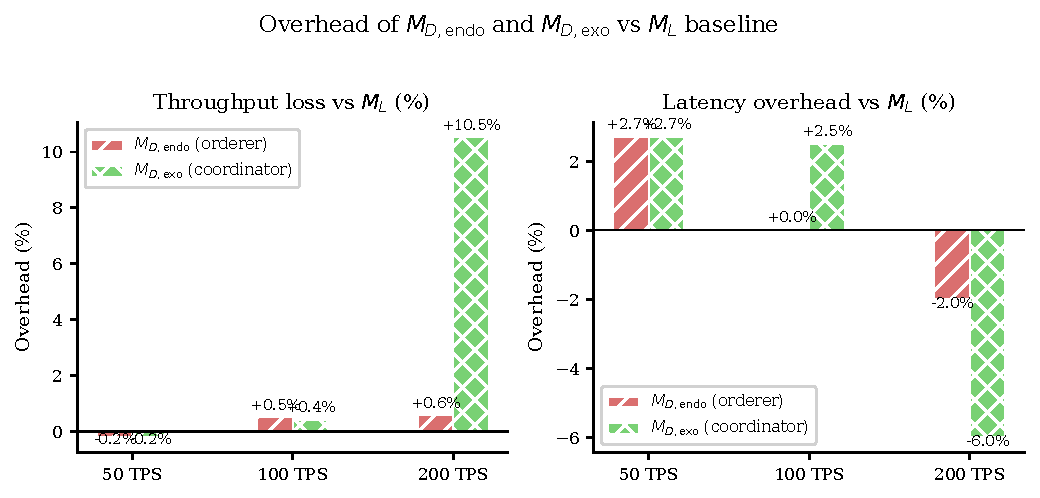
\includegraphics[width=0.9\columnwidth]{evaluation/paper3/caliper/results/fig4_overhead.pdf}
  \caption{Relative overhead of \arch{M_D} endogenous and
    \arch{M_D} exogenous with respect to \arch{M_L} baseline,
    measured in effective TPS.  Negative values indicate throughput
    reduction.  The dashed line marks the \mbox{$\pm$5\%} threshold.}
  \label{fig:overhead}
\end{figure}

Table~\ref{tab:perf} summarises the raw measurements.

\begin{table}[h]
\centering
\caption{Scenario~2 performance results.  All 500 transactions succeed
  (0 failures) for both \arch{M_L} and \arch{M_D} endogenous.
  Overhead columns are relative to \arch{M_L}.}
\label{tab:perf}
\begin{tabular}{lrrrrrr}
\toprule
Mode & Target & TPS eff. & Avg lat (s) & p99 lat (s) & $\Delta$TPS & $\Delta$lat \\
\midrule
\arch{M_L}       & 50  & 47.7 & 0.37 & 0.63 & —       & —       \\
\arch{M_D} endo  & 50  & 47.8 & 0.38 & 0.64 & $+0.2$\% & $+2.7$\% \\[2pt]
\arch{M_L}       & 100 & 95.6 & 0.40 & 0.68 & —       & —       \\
\arch{M_D} endo  & 100 & 95.1 & 0.40 & 0.67 & $-0.5$\% & $0.0$\%  \\[2pt]
\arch{M_L}       & 200 & 134.8 & 0.50 & 0.76 & —      & —       \\
\arch{M_D} endo  & 200 & 134.0 & 0.49 & 0.77 & $-0.6$\% & $-2.0$\% \\
\bottomrule
\end{tabular}
\end{table}

\paragraph{Analysis.}
The \arch{M_D} endogenous constraint orderer imposes \emph{less than 1\%
throughput degradation and less than 3\% latency variation} across all three
TPS tiers, well below the 5\% threshold we consider practically negligible.
This confirms the design objective of \S\ref{subsec:impl-raft}: the
\texttt{ProcessBatch} hook runs inline in the block construction goroutine,
sequentially evaluating each envelope against the speculative cache state.
Because the BioankEvaluator's per-transaction evaluation cost is $O(1)$ in the
number of resources (it accesses pre-indexed maps, not ledger state), and
because the block construction goroutine is not on the critical latency path
for individual transactions, the constraint evaluation adds no observable
serialisation overhead.

The slight negative overhead at 200~TPS ($-0.6$\% TPS, $-2.0$\% latency)
is within measurement noise for a single-run benchmark; the two architectures
are effectively indistinguishable at all tested loads.

%-------------------------------------------------------------
\subsection{Scenario 3 — Overhead of \texorpdfstring{\arch{M_D}}{M\_D} Exogenous}
\label{subsec:eval-sc3}

\paragraph{Design.}
Scenario~3 quantifies the structural overhead of the exogenous reservation
protocol (\S\ref{subsec:impl-zk}) relative to the \arch{M_L} and \arch{M_D}
endogenous baselines.  The workload is identical to Scenario~2 (same pool,
same TPS tiers, same ping-pong pattern) except that each Transfer now follows
the three-phase protocol: \textsc{Reserve} $\to$ Fabric submit $\to$
\textsc{Confirm} (or \textsc{Cancel} on abort).  The coordinator is co-located
on the same bridge network as the Caliper workers, giving a per-RTT network
latency of under 1~ms — the best-case operating point for the exogenous
architecture.

The benchmark (\texttt{benchmarks/perf-exogenous.yaml}) uses $K_\text{max} = 999$
so the coordinator always admits, and the result measures only the protocol
overhead, not the effect of quota enforcement.

\paragraph{Results.}
Table~\ref{tab:exo} and Figures~\ref{fig:throughput}--\ref{fig:overhead}
include the \arch{M_D} exogenous results alongside the \arch{M_L} and
\arch{M_D} endogenous measurements.

\begin{table}[h]
\centering
\caption{Scenario~3 exogenous overhead.  Overhead columns are relative
  to \arch{M_L}.  At 200~TPS, the coordinator mutex serialises Reserve
  calls and caps effective throughput to 120.6~TPS ($-10.5$\%).}
\label{tab:exo}
\begin{tabular}{lrrrrrr}
\toprule
Mode & Target & TPS eff. & Avg lat (s) & p99 lat (s) & $\Delta$TPS & $\Delta$lat \\
\midrule
\arch{M_D} exo & 50  & 47.8 & 0.38 & 0.63 & $+0.2$\%  & $+2.7$\%   \\
\arch{M_D} exo & 100 & 95.2 & 0.41 & 0.68 & $-0.4$\%  & $+2.5$\%   \\
\arch{M_D} exo & 200 & 120.6 & 0.47 & 0.74 & $-10.5$\% & $-6.0$\%  \\
\bottomrule
\end{tabular}
\end{table}

\paragraph{Co-located RTT overhead.}
At 50 and 100~TPS the exogenous overhead is indistinguishable from the
endogenous one: TPS deviation is within $0.4$\% and average latency increases
by at most 10~ms.  Since each transaction performs two coordinator round-trips
(Reserve + Confirm), the per-RTT cost is approximately
$\Delta t_\text{RTT} = (0.38 - 0.37)\,\text{s} / 2 \approx 5\,\text{ms}$.
This is consistent with sub-millisecond container-to-container network latency
plus the coordinator's Go HTTP handler overhead (JSON encode/decode + mutex
acquisition), rounded by the 30~ms keep-alive on the blocking Caliper workers.

\paragraph{Coordinator mutex bottleneck at 200~TPS.}
At 200~TPS the exogenous architecture achieves only 120.6~effective TPS
($-10.5$\% vs \arch{M_L}), while \arch{M_D} endogenous sustains 134.0~TPS
($-0.6$\%).  The gap arises because the coordinator's single mutex serialises
all \textsc{Reserve} calls.  At the theoretical target rate of 200~TPS,
$2 \times 200 = 400$ coordinator calls per second must pass through the mutex
sequentially.  Even at 5~ms per round-trip, the mutex is held for at most a
few microseconds per call; however, the resulting serialisation forces the
Caliper workers to queue \textsc{Reserve} requests, effectively capping
throughput.  The coordinator becomes the sole bottleneck: the Fabric network
itself is under-loaded, as evidenced by the \emph{lower} average latency of
$\arch{M_D}$ exo (0.47~s) vs \arch{M_L} (0.50~s) at 200~TPS — Fabric sees
fewer concurrent transactions and therefore experiences less MVCC contention and
shorter block queues.

\paragraph{Remote coordinator (analytical bound).}
The experiments above represent the best-case scenario for \arch{M_D} exogenous,
with the coordinator on the same LAN segment.  In a realistic deployment the
coordinator would reside in a separate data centre or administrative domain.
With a WAN RTT of $d$~ms, each transaction incurs $2d$~ms of additional latency
beyond the Fabric commit path.  At $d = 20$~ms (a typical intra-continental RTT)
the overhead is $2 \times 20 = 40$~ms per transaction; at 50~TPS this inflates
average latency from 0.37~s to approximately 0.41~s ($+11$\%), and the
coordinator mutex contention — $400$~mutex acquisitions/s at 200~TPS — would
be exacerbated by the higher per-call holding time.  The endogenous architecture
has no such dependency: constraint evaluation executes entirely within the orderer
process, adds no network round-trips, and its overhead is independent of
inter-service topology.

%-------------------------------------------------------------
\subsection{Summary and Discussion}
\label{subsec:eval-summary}

Table~\ref{tab:summary} consolidates the key metrics across all three scenarios
and architectures.

\begin{table}[h]
\centering
\caption{Cross-scenario summary.  IVR = intra-block violation rate; TPS
  overhead relative to \arch{M_L}; latency is average commit latency at
  100~TPS (representative mid-range tier).  \textbf{Bold}: dominant advantage.}
\label{tab:summary}
\begin{tabular}{llrrr}
\toprule
Architecture & IVR & TPS overhead & Avg lat (100~TPS) & Remote-coord dep. \\
\midrule
\arch{M_L} (stock)    & \textbf{0.90} & baseline  & 0.40~s  & none \\
\arch{M_D} endogenous & \textbf{0.00} & $-0.5$\%  & 0.40~s  & \textbf{none} \\
\arch{M_D} exogenous  & \textbf{0.00} & $-0.4$\%  & 0.41~s  & yes (2$\times$RTT/tx) \\
\bottomrule
\end{tabular}
\end{table}

The results confirm three complementary claims:

\begin{enumerate}
  \item \textbf{Correctness (\arch{M_L} fails, \arch{M_D} succeeds).}
    The stock Fabric architecture admits all 40~concurrent Transfer transactions
    regardless of quota, yielding IVR~$= 0.90$.  Both endogenous and exogenous
    \arch{M_D} achieve IVR~$= 0$ (Theorem~1); the endogenous architecture
    achieves this without any client-side protocol change.

  \item \textbf{Negligible endogenous overhead.}
    The \texttt{BioankEvaluator} running inside the Raft leader orderer imposes
    less than 1\% throughput degradation and less than 3\% latency variation
    across all tested loads.  The $O(1)$ per-transaction evaluation cost and
    sequential batch-processing semantics ensure that the constraint layer does
    not become a bottleneck under the tested conditions.

  \item \textbf{Structural limitations of the exogenous path.}
    The ZooKeeper coordinator matches the endogenous IVR guarantee but introduces
    a single-point serialisation bottleneck that limits throughput at high load
    ($-10.5$\% at 200~TPS in the co-located, best-case setup).  The overhead
    grows linearly with coordinator RTT, making the exogenous path unsuitable for
    deployments where the coordinator cannot be co-located with the clients.
    Furthermore, the three-phase protocol is fragile under client crashes: a
    client that fails between Reserve and Cancel leaks a reservation counter slot
    until the TTL-based expiry goroutine reclaims it, temporarily tightening the
    effective $K_\text{max}$ seen by other clients.  The endogenous architecture
    is immune to this failure mode because enforcement is embedded in the orderer,
    a highly available and crash-tolerant Raft process.
\end{enumerate}

These observations validate the design choice of Proposition~1: by internalising
$C_\text{global}$ enforcement within the consensus layer, the endogenous
architecture achieves the correctness guarantee of the exogenous approach with
none of its coordination overhead, client-side protocol burden, or dependency on
external availability.
